%\RequirePackage{lineno}
%\documentclass[aps, prc, reprint, amsmath, groupedaddress, nofootinbib]{revtex4-1}
\documentclass[twocolumn,aps,superscriptaddress,showpacs,nofootinbib,floatfix]{revtex4}
\usepackage{float}
\usepackage{listings}
\usepackage[utf8]{inputenc}
\usepackage{hyperref}
\usepackage{amsmath}
\usepackage{amssymb}
\usepackage{amsfonts}
\usepackage{tabularx}
\usepackage{booktabs}
\usepackage{graphicx}
\usepackage{subfigure}
\usepackage{color}
%\usepackage[switch]{lineno}
\usepackage{diagbox}
\usepackage{multirow}
\usepackage{bm}
\usepackage[inline]{enumitem}
%\usepackage{setspace}
\usepackage[T2A,T1]{fontenc}
\lstset{language=[LaTeX]TeX,keywordstyle=\color{red},showspaces=true,breaklines=true,breakatwhitespace=true,basicstyle=\small\tt,commentstyle=\color{white},frame=single,framerule=0pt,backgroundcolor=\color{yellow}}
\graphicspath{{fig/}}
\definecolor{theblue}{RGB}{0,50,230}

\usepackage{hyperref}
\hypersetup{
  colorlinks=true,
  linkcolor=theblue,
  citecolor=theblue,
  urlcolor=theblue
}
\newcommand{\pT} {\ensuremath{p_{\mathrm{T}}}}
\def\simge{\stackrel{>}{\sim} }
\def\simle{\stackrel{<}{\sim} }
\newcommand{\nch}{N_\text{ch}}
\newcommand{\sqrts}{\sqrt{s_{NN}}}
\newcommand{\T}{\tilde{T}}
\newcommand{\paddedhline}{\noalign{\smallskip}\hline\noalign{\smallskip}}
\newcommand {\avg}[1]{\ensuremath{\langle\kern-1.0pt\langle#1\rangle\kern-1.0pt\rangle}}
\newcommand{\dnchdy}{dN_\text{ch}/d\eta}
\newcommand{\dndypP}{dN_\text{pPb}/d\eta}
\newcommand{\dndyPP}{dN_\text{PbPb}/d\eta}
\newcommand{\dphi}    {\ensuremath{\Delta\phi}}
\newcommand{\x}{\mathbf x}
\newcommand{\y}{\mathbf y}
\newcommand{\z}{\mathbf z}
\newcommand{\trans}{^\intercal}
\newcommand{\La}{\langle}
\newcommand{\Ra}{\rangle}
\newcommand{\pttrg}      {\ensuremath{\pt^{a}}\xspace}
\newcommand{\ptass}      {\ensuremath{\pt^{b}}\xspace}
\newcommand{\avgevvn}[1]{\left\langle{#1}\right\rangle}
\newcommand{\Qf}[2]{\frac{\tilde{Q}_{#1}^{#2}}{|\tilde{Q}_{#1}^{#2}|}}
\newcommand{\Qfs}[2]{\frac{\tilde{Q}_{#1}^{*#2}}{|\tilde{Q}_{#1}^{#2}|}}
\newcommand{\lr}[1]{\left\langle #1\right\rangle}
\def\eq{{\,=\,}}
\newcommand{\avgev}[1]{\left\langle{#1}\right\rangle}
\def\bra{\langle}
\def\ket{\rangle}
\newlength\cmsFigWidth
\def\tq{T_q}
\def\ts{T_s}
\def\pt{p_T}
\def\bq{\begin{eqnarray}}
\def\eq{\end{eqnarray}}

%%%%%%%%%%%%%%%%%%%%%%%%%%%%%%%%%%%%%%%%%%%%%%%%%%%%%%
\usepackage[normalem]{ulem}  % \sout{old text} for strikeout
%\usepackage[dvips]{color} % For blue in-text com ments and additions
\newcommand{\com}[1]{{\sf\color[rgb]{0,0,1}{#1}}}
\newcommand{\modi}[1]{{\sf\color[rgb]{1,0,0}{#1}}}
\newcommand{\ans}[1]{{\sf\color[rgb]{0,1,0}{#1}}}
\renewcommand\sout{\bgroup \color{red} \ULdepth=-.5ex \ULset}
%%%%%%%%%%%%%%%%%%%%%%%%%%%%%%%%%%%%%%%%%%%%%%%%%%%%%

\newcommand{\blue}[1]{{\color{blue}{#1}}}
\newcommand{\green}[1]{{\color{green}{#1}}}
\newcommand{\red}[1]{{\color{red}{#1}}}


\begin{document}
%\linenumbers
%%%%%%%%%%%%%%%%%%%%% Title %%%%%%%%%%%%%%%%%%%%%%

\title{Centrality and transverse momentum dependence of hadrons in Au+Au collisions at BES energy region}

%%%%%%%%%%%%%%%%%%%% Authors %%%%%%%%%%%%%%%%%%%%%
\author{Huanjing Gong}
\author{Zhizhen Ye}
\author{Guiqi Liu}

\affiliation{Department of Physics, Sichuan University, Chengdu 610064, China}
\author{Lilin Zhu}\email{zhulilin@scu.edu.cn}


%%%%%%%%%%%%%%%%%%%% Abstract %%%%%%%%%%%%%%%%%%%%%
\begin{abstract}
The transverse momentum spectra of seven identified hadrons ($\pi$, K, p, $\Lambda$, $\phi$, $\Xi$, $\Omega$) produced in Au+Au collisions in the BES energy region have been investigated in the framework of the recombination model (RM). The investigation has testified that the results are extended successfully to the $p_T$ distributions in the energy range of Beam-Energy Scan (BES) Program at the Relativistic Heavy-Ion Collider (RHIC) over wide ranges of $p_T$, particularly in the region of low $p_T$. Our study shows great agreement between theoretical results and experimental data with only two parameters. With all of dependence taken into account, the exciting results shows good similarity of final state hardons in quite a wide collision energy from $\sqrt{s_{NN}}=7.7$ GeV to $\sqrt{s_{NN}}=5.02$ TeV. Besides, valon model is expected to apply to K production in Au+Au collisions and our attempt is exhibited in the followings.
%Soft, semihard and hard partons all play important roles in our model and are uniformly treated for all hadrons produced.
\end{abstract}

\pacs{25.75.Nq, 25.75.Ld}
\keywords{}
\maketitle

\section{introduction}
Quark gluon plasma (QGP) is the main state of universe in the earlier period after big bang, which makes a big difference on the evolution of cosmos. Strongly interacting matter composed of hadronic constituents, like proton and neutron, undergoes the phase transition to QGP in a high-energy-density and high-temperature phase where the quantum chromodynamics (QCD) phase diagram exhibits in high-energy heavy-ion collision experiments. Experimentally, the final state observables is the crucial tools as figuring out the mechanism of recombination of particles. Hwa-Yang recombination model is adopted to describe the universal productions for all identified hadrons over wide ranges of transverse momenta in heavy-ion collisions pretty well\cite{2u}. Moreover, in order to map out the phase diagram of the QCD matter, a Beam Energy Scan (BES) program has been initiated at RHIC with Au+Au collisions at $\sqrt{s_{NN}}=7.7\sim39$ GeV \cite{STAR:2015vvs}. In this paper, seven identified hadrons ($\pi$, K, p, $\Lambda$, $\phi$, $\Xi$, $\Omega$) are included to expand our investigation in beam energy region at $\sqrt{s_{NN}}=7.7\sim39$ GeV and centrality has been taken into account. 

In Section~\ref{RM2}, we will introduce the formulation of recombination to calculate the $p_T$ distribution, which mainly include thermal and shower partons. The exponential behavior of thermal partons is valid over wide ranges of $p_T$ while show parton distribution is integrated over jet momentum and summed over all jets. In the BES region, the momentum of quarks is much lower than in the intermediate region, resulting in the dominant $\mathcal T\mathcal T$ and $\mathcal T\mathcal T\mathcal T$ components and the negligible components associated with $\mathcal S$. Therefore, we show the huge difference in several orders of magnitude in Section~\ref{RM2} and then in Section~\ref{DOH4} we only consider the $\mathcal T\mathcal T$ and $\mathcal T\mathcal T\mathcal T$ components that play the dominant role in fact.

In Section~\ref{BS3}, we follow up the notion in \cite{4u} to consider a baryon spectra to obtain two coefficients which can be calculated in \cite{3c} by linearly fitting the experimental data of spectra. And in Section~\ref{DOH4}, we will give the formulation of transition between baryon spectra and $p_T$ distribution of hadrons to derive the significant parameter normalization $C_j$ and inverse slope $T_j$. Subsequently, in Section~\ref{results5} we display the results from our study on the centrality dependence of transverse momentum spectra of seven identified hadrons in Au+Au collisions at $\sqrt{s_{NN}}=7.7\sim39$ GeV.

Besides, we have studied hadronic collisions in the valon-recombination model (VRM) \cite{5i}, which is expected to fix the slight deviation in Section~\ref{RM2} for kaon. In Section~\ref{VM6}, valon model is presented to calculate proton inclusive distributions with two parameters. What's new is that we adopt a rough approximation that one of the two baryons in hadronic collisions can be simply regarded as the combination of protons and neutrons so that particle production in AA collisions can be calculated, while the processes, not only of pp, but also of pA collisions have been checked with valon-recombination model \cite{6c}. Finally, section~\ref{summary7} summarizes the results and makes a conclusion in terms of the present work, as well as the expectation of implementation of valon model in Au+Au collisions. 



%The ultimate goal of the physics program with ultrarelativistic nucleus-nucleus collisions is to understand the properties of strongly interacting matter under extreme conditions of high temperature and density. Quantum Chromodynamics (QCD) predicts that at sufficiently high density strongly interacting matter undergoes a phase transition from a state of hadronic constituents to quark and gluon plasma (QGP). One of the most promising signals of the deconfinement is related to particular properties of transverse momentum spectra of final hadrons. The conventional methods to describe hadron production in heavy-ion collisions are by use of hydrodynamical model for transverse momentum $p_T<2$ GeV/c \cite{kh, tat, gjs, hydroepjczhao} and by jet fragmentation for $p_T>8$ GeV/c \cite{pq2, mt, jet}. In the intermediate region neither approaches are applicable, while parton recombination or coalescence (ReCo) model in heavy-ion collisions has been found to be more relevant \cite{hy0, gkl, fmnb}. The large baryon-to-meson ratio is an observed phenomenon that is successfully explained by ReCo to fill the gap \cite{hy0, gkl, fmnb, hz2, Zhu:2014csa}. 

%Despite differences in detail, the basic ideas in the three formulations of ReCo are very similar \cite{hy0, gkl, fmnb}. In this study, the Hwa-Yang recombination model (RM) is adopted \cite{hy0}. It is formulated in one dimension along the direction of recombination on the basis that non-collinear partons have low probability of coalescence, but it incorporates fragmentation as a component of recombination so that there is a smooth transition from low to high $p_T$. Within the framework of RM, the transverse momentum and centrality dependence of hadron production in Au+Au collision at $\sqrt{s_{NN}}=200$ GeV at RHIC were well reproduced \cite{hz2}. It is found that the recombination of thermal and shower partons is the major component for intermediate $p_T$ region. In heavy-ion collisions above 2 TeV, the density of minijets produced by semihard scatterings of partons can be so high that the conventional  treatment of such collisions may be inadequate. Recently, the spectra of hadrons produced in central Pb+Pb collisions at $\sqrt{s_{NN}}=2.76$ TeV has been studied with $p_T$ up to 20 GeV/c by the recombination model. It is found that the minijets are abundantly produced at LHC compared with RHIC \cite{Zhu:2014csa}. These previous studies \cite{hz2, Zhu:2014csa} have revealed that the formation of hadrons at intermediate $p_T$ region is sensitive to the momentum degradation of the hard and semihard partons. Furthermore, due to the geometrical configuration of colliding system, the momentum degradation from the initial parton momentum to the final momentum at the medium surface is different for Au+Au and Pb+Pb collisions. Even for the same colliding system, the momentum degradation is not the same for different colliding energies. We will give more discussion later.
%
%In heavy-ion collisions there are various theoretical issues related to minijets that have not yet evolved to a mature subject with general acceptance. The medium effects on semihard partons are important but hard to make precise, and the hadronization process is still controversial. The shower partons not only depend on the momentum degradation in the medium, but also can be hadronized through various channels, such as recombination with thermal partons on the one hand and with other shower partons on the other. At LHC the high density of jets enables the possibility of shower partons from different jets overlapping in common spatial proximity so that the contribution from their coalescence cannot be ignored. We have studied the minijet contribution to the central Pb+Pb collisions at $\sqrt{s_{NN}}=2.76$ TeV and reproduce the hadron production very well \cite{Zhu:2014csa}. Therefore, we will extend the investigation of the $p_T$ spectra of identified hadrons to non-central collisions in Pb+Pb collisions at both $\sqrt{s_{NN}}=2.76$ and 5.02 TeV with the recombination model in this study and conclude with a summary on our general view of the hadronization process in nuclear collisions.
%
%The paper is organized as follows: In Section~\ref{RM}, we briefly review the basic framework of Hwa-Yang recombination model, including the inclusive distribution of minijets. The formalisms of parton combination for pion, proton and kaon are shown  in Section~\ref{IDH}. In Section~\ref{results}, we show results from our study on the centrality dependence of transverse momentum spectra of seven identified hadrons in Pb+Pb collisions at $\sqrt{s_{NN}}=2.76$ and 5.02 TeV. Finally, section~\ref{summary} summarizes the results and gives the conclusion from the present study.

\section{formulation of quark recombination}\label{RM2}
As recombination model mentioned \cite{2u,3c,4u,5i}, we start from the universal formalism in brief to calculate the $p_T$ distribution. The basic framework by definition emphasizes that thermal and shower partons in jets or minijets at midrapidity undergo the processes of recombination, resulting in the production of mesons and baryons. Therefore, the formula of distributions naturally is a convolution of the parton distribution with the recombination function over $\eta$ at midrapidity
\begin{eqnarray}
\hspace{-0.5cm}p^0{dN^M\over dp_T}&=&\int {dp_1\over p_1}{dp_2\over p_2} F_{q_1\bar q_2}(p_1,p_2) R_{q_1\bar q_2}^M(p_1,p_2,p_T), 
\label{2.1}
\end{eqnarray}
\begin{eqnarray}
\hspace{-1.5cm}p^0{dN^B\over dp_T}&=&\int {dp_1\over p_1}{dp_2\over p_2}{dp_3\over p_3} F_{q_1q_2q_3}(p_1,p_2,p_3)\nonumber\\ 
&&\times {R}_{q_1q_2q_3}^B(p_1,p_2,p_3,p_T),   
\label{2.2}
\end{eqnarray}
in which $q_i$ means the transverse momenta of quarks and $R^{M}$ and $R^{B}$ represents the recombination functions for mesons and baryons. Then, the paton distributions are partitioned into several components
\begin{eqnarray}
F_{q_1\bar q_2}=\mathcal T\mathcal T+\mathcal T\mathcal S+\mathcal S\mathcal S,
\label{2.3}
\end{eqnarray}
\begin{eqnarray}
F_{q_1 q_2 q_3}=\mathcal T\mathcal T\mathcal T+\mathcal T\mathcal T\mathcal S+\mathcal T\mathcal S\mathcal S+\mathcal S\mathcal S\mathcal S,
\label{2.4}
\end{eqnarray}
where $\mathcal{T}$ and $\mathcal{S}$ represent the invariant distributions for thermal and shower partons in terms of momenta just before hadronization, respectively. At BES energy region, as seen later, $\mathcal{S}$ components are small enough to neglect while the dominant $\mathcal{TT}$ and $\mathcal{TTT}$ components are mainly calculated, owing to the low transverse momenta $p_i$ caused by the low energy of the colliding system.

A simple exponential form is assumed statistically for the thermal parton distribution
\begin{eqnarray}
\mathcal T_j(p_i)=p_i\frac{dN_j}{dp_i}=C_jp_ie^{-p_i/T_j},
\label{2.5}
\end{eqnarray}
where the subscript $j$ denotes quark ($u, d, s$). Since the mass of $s$ is different from $(u, d)$, to distinguish them, we use $q$ to denote $(u, d)$. The normalization factor $C_j$, dependent of the number of participants $N_{part}$ and $\sqrt{s_{NN}}$, has the dimension of inverse momentum and the inverse slope $T_j$, only dependent of $\sqrt{s_{NN}}$, is determined by fitting the experimental data of spectra at low $p_T$\cite{3c} and includes the dissipative effects of minijets on the expanding medium at all times of the evolution of the plasma\cite{4u}. Furthermore, we use the universal formula for the energy dependence of $T_j$ in \cite{4u},
\bq
T_q(s)&=&T_1 f(s), \qquad  T_s(s)=T_2 f(s),    \label{2.6}  \\
f(s)&=&{\sqrt s}\ ^\beta, \qquad  {\sqrt s} \text{ in TeV}
\label{2.7}
\eq
with the slightly different in \cite{4u} but same in \cite{2u} parameters
\bq
T_1=0.39\ {\rm GeV/c}, \quad T_2=0.51\ {\rm GeV/c}, \quad \beta=0.105.  \label{2.8}
\eq
Hereafter, $\sqrt{s}$ in the formulae denotes $\sqrt{s_{NN}}$. The values of $T_j$ are given in Table \ref{tab1}. 
\begin{table}
\tabcolsep0.13in
%\begin{spacing}{1.3}
\begin{tabular}{cccccc}
\hline
\hline
 $\sqrt{s}$ (GeV) &7.7 &11.5 &19.6 &27 &39\\ 
 \hline
$T_q$ (GeV) & 0.234 & 0.244 &0.258 &0.267 &0.277\\
$T_s$ (GeV) &0.306 &0.319 &0.338 &0.349 &0.363\\
 \hline
  \hline
 \end{tabular}
 %\end{spacing}
 \caption{Parameters $T_q$ and $T_s$ for Au+Au collisions at $\sqrt{s}=7.7, 11.5, 19.6, 27$ and 39 GeV, respectively.} 
 \label{tab1}
 \end{table} 

Now, we just give the formula of the shower parton distribution, associated with the fragmentation function and distribution of jet, and more details have been explicated in \cite{2u} because component $\mathcal{S}$ is not needed and interested at BES region.
\begin{eqnarray}
{\cal S}^j(p_{2}, c)=\int {dq\over q}\sum_i \hat F_i(q, c) S_i^j(p_2, q).  \label{2.9}
\end{eqnarray}

Fig.\ref{fig1} shows the transverse momentum spectra for seven identified hadrons ($\pi$, K, p, $\Lambda$, $\phi$, $\Xi$, $\Omega$) in Au+Au collisions at $\sqrt{s_{NN}}=39$ GeV and the collision of 0-5\%. According to the $p_T$ spectra, $\mathcal{TT}$ and $\mathcal{TTT}$ components are seen to be absolutely dominant so the effects of minijets and jets can be ignored, whereupon in Secs. \ref{BS3} and \ref{DOH4} we only talk over the dominant components. And another thing worthy of attention is that the theoretical curves fit remarkably the experimental data by two parameters $C$ and $C_s$ given below except for the kaon distribution. 
\bq
C_{q}=38.0, \quad C_{s}=10.7. \label{2.10} 
\eq
Hence, we attempt to utilize the valon-recombination model(VRM) to improve the transverse momentum distribution of K produced in Au-Au collision in Section~\ref{VM6}.
\begin{figure*}[pht]
  \includegraphics[width=0.9\textwidth]{pic1.png}
  \caption{Transverse momentum spectra of $\Xi$ (a), proton (b), $\Omega$ (c), $\Lambda$ (d), $\pi$ (e), $\phi$ (f) and K (g) from the recombination model at midrapidity for Au+Au collisions at $\sqrt{s_{NN}}=39$ GeV and centralities of 0-5\%. The experimental data are taken from Ref. \cite{STAR:2019bjj,STAR:2017sal,STAR:2015vvs}.}
\label{fig1}
\end{figure*}

To correspond to the following section, a simplified parton distribution should be gained, which specifically presented in Section~\ref{DOH4}. Now we can write the recombination function as
\begin{eqnarray}
{{\it R_{h}}(p_1,p_2,p_3,p_T)=W_{h}(y_1,y_2,y_3)\delta\bigg{(}\sum\limits_{i}y_i-1\bigg{)},}
\label{2.11}
\end{eqnarray}
where $y_i = p_i/p_T$, which is the momentum fraction of the $i$th quark in the hadron $h$, and for proton $W_p (y_1,y_2,y_3)$ has been studied in the valon model\cite{Hwa:2002mv} discussed in Section~\ref{VM6}. Then there follows the condition for baryons and the figure for mesons also follow the notion. On the basis that the average momentum fraction ⟨$y_i$⟩ of each quark in a hyperon is 1/3, we simplify Eq.\ref{2.11} further by the approximation for all $h$\cite{4u}, 
\begin{eqnarray}
	{{\it R_{h}}(p_1,p_2,p_3,p_T)={\text g}_h \prod \limits_{i=1}^3\delta(p_i/p_T-1/3),}
	\label{2.12}
\end{eqnarray}
where $g_h$ is a numerical factor depends only on hadron. Substituting Eqs.\ref{2.4},\ref{2.5} and \ref{2.12} into Eq.\ref{2.2}, the universal baryon distribution is
\begin{eqnarray}
	p^0{d\overset{\bm-}{N}\over dp_T}&=&\bigg(\prod \limits_{i=1}^3 C_i \bigg) g_h p_T^3 \text{exp}\bigg[-\frac{p_T}{T_h}\bigg],   
	\label{2.13}
\end{eqnarray}
where $T_h$ satisfies the following identification:
\begin{eqnarray}	T_h=\frac{1}{3}\sum\limits_i\frac{1}{T_i}=\frac{1}{3}\Big( \frac{3-n_s}{T_q}+\frac{n_s}{T_s} \Big),
	\label{2.14}
\end{eqnarray}
where $n_s$ is the number of strange quarks in $h$. At mid-rapidity considered here and in \cite{2u}, we have $p^0\approx m_T^h$, where $m_T^h=(m_h^2+p_T^2)^{1/2}$, $m_h$ being the mass of baryon $h$. 
%Let us start by recalling the basic elements of the recombination model. Our study here is limited to the midrapidity and all the formulae are averaged over the azimuthal angles. Therefore, the invariant distributions of mesons and baryons are, which are averaged over $\eta$ at midrapidity \cite{hy0, hy1, hz1, hz2, Hwa:2009tx, Zhu:2014csa}
%\begin{eqnarray}
%\hspace{-0.5cm}p^0{dN^M\over dp_T}&=&\int {dp_1\over p_1}{dp_2\over p_2} F_{q_1\bar q_2}(p_1,p_2) R_{q_1\bar q_2}^M(p_1,p_2,p_T), 
%\label{2.1}
%\end{eqnarray}
%\begin{eqnarray}
%\hspace{-1.5cm}p^0{dN^B\over dp_T}&=&\int {dp_1\over p_1}{dp_2\over p_2}{dp_3\over p_3} F_{q_1q_2q_3}(p_1,p_2,p_3)\nonumber\\ 
%&&\times {R}_{q_1q_2q_3}^B(p_1,p_2,p_3,p_T),   
%\label{2.2}
%\end{eqnarray}
%with the transverse momenta of coalescing quarks $p_i$. $R^{M}$ and $R^{B}$ are the recombination functions (RFs) of the corresponding quarks for mesons and baryons, respectively. The parton distributions can be partitioned into various components, represented symbolically by
%\begin{eqnarray}
%F_{q_1\bar q_2}=\mathcal T\mathcal T+\mathcal T\mathcal S+\mathcal S\mathcal S,
%\label{2.3}
%\end{eqnarray}
%\begin{eqnarray}
%F_{q_1 q_2 q_3}=\mathcal T\mathcal T\mathcal T+\mathcal T\mathcal T\mathcal S+\mathcal T\mathcal S\mathcal S+\mathcal S\mathcal S\mathcal S,
%\label{2.4}
%\end{eqnarray}
%where $\mathcal{T}$ and $\mathcal{S}$ represent the invariant distributions for thermal and shower partons just before hadronization, respectively.
%The former contains the medium effect, while the latter is due to semihard and hard scattered partons. The consideration of shower partons is a unique feature of our model to recombination, which is empowered by the possibility to include fragmentation process as $\mathcal S\mathcal S^{1j}$ or $\mathcal S\mathcal S\mathcal S^{1j}$ recombination.
%For the contribution with two or three shower partons, we need to take into account their sources. For a visualization of the various processes, we refer to the schematic diagrams in Ref. \cite{Zhu:2014csa}.  The shower partons in $\mathcal S\mathcal S$ and $\mathcal T\mathcal S\mathcal S$ can be from the same jet or two jets. For $\mathcal S\mathcal S\mathcal S$, only the contributions of $\mathcal S\mathcal S\mathcal S^{1j}$ and $\mathcal S\mathcal S\mathcal S^{2j}$ are included in this study, because the contribution from $\mathcal S\mathcal S\mathcal S^{3j}$ referring to three shower partons from three jets is highly suppressed.
%
%The thermal parton distribution is assumed to have a simple exponential form \cite{hy0, Zhu:2014csa}
%\begin{eqnarray}
%\mathcal T_j(p_i)=p_i\frac{dN_j}{dp_i}=C_jp_ie^{-p_i/T_j},
%\label{2.5}
%\end{eqnarray}
%where the subscript $j$ denotes quark ($u, d, s$). Since the mass of $s$ is different from $(u, d)$, to distinguish them, we use $q$ to denote $(u, d)$. The normalization factor $C_j$ has the dimension of inverse momentum. 
%
%We remark with emphasis that the symbols ($\cal T$, $T_j$) and word (thermal) used here are carried over from previous work \cite{hy0, Zhu:2014csa} without modification in order to preserve the continuity of the mathematical formalism of the RM. However, the physical content of the model before hadronization may evolve with increasing energy and with better understanding of the physical processes. In particular, at the collision energies that we consider here, rapid equilibration would not be realistic, since some hard and semi-hard partons can take over 5 fm/c to traverse the transverse dimensions of the initial system, whereby they deliver considerable energy to the expanding system. Even though the bulk system may not be fully equilibrated at the time of hadronization, we still refer to the soft sector as “thermal”, so as to distinguish it from the harder sector that includes semi-hard or hard partons that produce the shower partons. The exponential form in Eq. (\ref{2.5}) is assumed on phenomenological grounds with the value of $T_j$ to be adjusted to fit the new data. The parameter $T_j$ is referred to as inverse slope, which, we stress, is not temperature, a term that is suitable only for a fully equilibrated thermal system. What is remarkable is that the exponential form in Eq. (\ref{2.5}) provides excellent fits of the data with the inverse slope being grossly different from the conventional temperature of thermalized systems at lower collision energies.
%
%A universal formula for the energy dependence of $T_j$ was obtained in Ref. \cite{Hwa:2018qss},
%\bq
%T_q(s)&=&T_1 f(s), \qquad  T_s(s)=T_2 f(s),    \label{2.6}  \\
%f(s)&=&{\sqrt s}\ ^\nu,   \label{2.7}
%\eq
%with the parameters
%\bq
%T_1=0.35\ {\rm GeV/c}, \quad T_2=0.46\ {\rm GeV/c}, \quad \nu=0.105.  \label{2.8}
%\eq
%For simplicity, we have used $\sqrt{s}$ to replace $\sqrt{s_{NN}}$. It should be pointed out that $\sqrt{s}$ in Eq. (\ref{2.7}) is scaled by 1 TeV and dimensionless. The values of $T_j$ for $\sqrt{s}=2.76$ and 5.02 TeV are given in Table \ref{tab1}. 
%
%\begin{table}
%\tabcolsep0.25in
%%\begin{spacing}{1.3}
%\begin{tabular}{ccc}
%\hline
%\hline
% $\sqrt{s}$ (TeV) &2.76 &5.02\\ 
% \hline
%$T_q$ (GeV) & 0.39 & 0.415 \\
%$T_s$ (GeV) &0.51 &0.545 \\
% \hline
%  \hline
% \end{tabular}
% %\end{spacing}
% \caption{Parameters $T_q$ and $T_s$ for Pb+Pb collisions at $\sqrt{s}=2.76$ and 5.02 TeV, respectively.} 
% \label{tab1}
% \end{table}
% 
%As discussed in Ref. \cite{Zhu:2014csa}, the shower parton distribution is given by
%\begin{eqnarray}
%{\cal S}^j(p_2)=\int {dq\over q}\sum_i \hat F_i(q) S_i^j(p_2, q),  \label{2.9}
%\end{eqnarray}
% where  $S_i^j(p_2, q)$ is the shower parton distribution (SPD) in a jet of type $i$ fragmentating into a parton of type $j$ with momentum fraction of $p_2/q$. It is determined by the fragmentation functions (FFs) known from analyzing leptonic processes on the basis that hadrons in a jet are formed by recombination of the shower partons in the jet \cite{hy4}. Once the SPDs are known, one can give a more complete description of hadronization, especially for the nuclear collisions. After including the centrality dependence, Eq. (\ref{2.9}) should be modified as
%\begin{eqnarray}
%{\cal S}^j(p_2, c)=\int {dq\over q}\sum_i \hat F_i(q, c) S_i^j(p_2, q).  \label{3.6}
%\end{eqnarray}
%$\hat{F_i}(q, c)$ is the distribution of hard and semihard parton of type $i$ at the medium surface after momentum degradation while transversing the medium. At a specified centrality $c$ (e.g. $c=0.05$ stands for $0-10\%$ centrality) it is defined as 
% \begin{eqnarray}
%\hat F_i(q, c)&=&\frac{1}{2\pi}\int d\phi\int d\xi P_i(\xi, \phi, c) \\ \nonumber
%&&\times\int dkkf_i(k, c)G(k, q, \xi), \label{2.10}
%\end{eqnarray}
%$P_i(\xi, \phi, c)$ is the probability for parton $i$ having a dynamical path length $\xi$ at angle $\phi$ initiated at position $(x_0, y_0)$, weighted by the nuclear overlap function and integrated over all $(x_0, y_0)$. The connection between geometry and dynamics is imbedded in $P_i(\xi, \phi, c)$. The dynamical path length $\xi$ is proportional to the geometrical path length $l$. Therefore, $P_i(\xi, \phi, c)$ can be written as
%\begin{eqnarray}
%P_i(\xi, \phi, c) =\int dx_0dy_0Q(x_0, y_0, c)\delta(\xi-\gamma_i l).
%\end{eqnarray}
%where $Q(x_0, y_0, c)$ is the probability that a hard (or semihard) parton is produced at $(x_0, y_0)$, which can be calculated from nucleon thickness functions \cite{hz2, Hwa:2009tx}. The factor $\gamma_i$ is introduced to account for the effects of jet quenching in the medium that results in additional parton degradation due to the soft partons created. The dependence of that factor on the colliding energy will be considered below. As stated in Ref. \cite{Hwa:2009tx}, all physical lengths are in units of the effective nuclear radius $R_A$, so the geometrical path length $l$ is numerical in that unit, whereas $\gamma_i$ has the characteristic of inverse length, resulting in $\xi$ being dimensionless, although it has been referred to as dynamical path length.
%
%The function $f_i(k, c)$ is the density of parton $i$ in the phase space $kdk$. For central collisions, the initial momentum distribution $f_i(k, c)$ was parametrized as \cite{sgf}
%\begin{eqnarray}
%f_i(k, 0.05)=K\frac{A}{(1+k/B)^{n}}. 
%\label{2.12}
%\end{eqnarray}
%For Pb+Pb collisions at 2.76 TeV, the parameters in Eq. (\ref{2.12}) were obtained by logarithmic interpolations of the parameters $\ln A$, $B$ and $n$ between Au+Au collisions at 200 GeV and Pb+Pb collisions at 5.5 TeV with $K=2.5$, as shown in Ref. \cite{Zhu:2014csa}. Following the same approach, we can get the parameters for central Pb+Pb collisions at 5.02 TeV listed in TABLE \ref{tab2}. Taking into account the centrality dependence, the minijet distribution can be calculated by
%\begin{eqnarray}
%f_i(k, c) = \frac{T_{AA}(c)}{T_{AA}(0.05)}f_i(k, 0.05).
%\end{eqnarray}
%The nuclear thickness function $T_{AA}(c)$ for Pb+Pb collisions are available in Ref. \cite{Abelev:2013qoq}.
%
%For the momentum degradation function $G(k, q, \xi)$ due to energy loss, as discussed in Ref. \cite{Zhu:2014csa}, we take the simple form 
%\begin{eqnarray}
%G(k, q, \xi)=q\delta(q-ke^{-\xi}) \label{2.11}
%\end{eqnarray}
% as an adequate approximation of the complicated processes involved in the parton medium interaction. 
% 
%Therefore, $\hat{F}_i(q, c)$ can be calculated once $\gamma_i$ is known. Unfortunately, we cannot calculate $\gamma_i$ directly, since it is a factor that approximates the effects of energy loss during the passage of the parton through the non-uniform and expanding medium that is not thermalized due to the energy degradation processes of all the semi-hard partons produced throughout the medium. Those effects have not been successfully treated from first principles. We have used $\gamma_i$ as a phenomenological factor with parameters adjusted to fit the data. Since quarks and gluons lose their energies at different rates when they go  through the medium, we assumed that $\gamma_q=\gamma_g/2=0.07$ and obtained excellent fits for hadron spectra in Au+Au collisions at $\sqrt{s_{NN}}=200$ GeV  \cite{hz2} . For the momentum degradation at LHC, the $\gamma_i$ factor cannot remain the same as that at RHIC due to many more minijets produced and the different geometrical configuration of colliding system. For Pb+Pb collisions, we parametrized it as \cite{Zhu:2014csa}
%\begin{eqnarray}
%\gamma_g(q)=\frac{\gamma_0}{1+(q/q_0)^2}.
%\end{eqnarray}
%The parameters $\gamma_0$ and $q_0$ are determined by fitting the spectra in the intermediate $p_T$ region. For Pb+Pb collisions at 2.76 TeV, we have obtained $\gamma_0=2.8$ and $q_0=7$ GeV/c \cite{Zhu:2014csa}. Their values for  Pb+Pb collisions at 5.02 TeV will be discussed in Sec. \ref{results}.
%
%\begin{table*}
%\tabcolsep0.2in
%%\arraycolsep1in
%\begin{tabular}{|c|c|c|c|c|c|c|}
%\hline
% & $g$ &  $u$ &  $d$ & $\bar u$ &  $\bar d$  &s, $\bar s$\\ 
% \hline
% $A$ [$10^4$/GeV$^2$] & 11.2 &2.02 &2.28 &0.42 &0.40& 0.154\\
% $B$ [GeV]& 0.80 &0.59 &0.58 &0.75 &0.76 &0.93\\
% $n$ & 5.68 &5.31 &5.29 &5.52 &5.53 &5.63\\
% \hline
% \end{tabular}
% \caption{Parameters for $f_i(k, 0.05)$ in Eq.\ (\ref{2.12}) for central Pb+Pb collisions at $\sqrt{s}=5.02$ TeV.} 
% \label{tab2}
% \end{table*}

\section{baryon and meson spectra}\label{BS3}
With the results above, we consider to stay close to the data and search for a description that is applicable to all baryons and mesons to obtain the universal formalism and parameters\cite{4u}. Firstly, we transform the $p_T$ spectra to linear formula for baryons and mesons respectively
\begin{eqnarray}
B_h(s,N_{part},p_T)=\frac{m_T^h}{p_T^2} {d\overset{\bm-}{N_h}\over p_T dp_T}(s,N_{part}),
\label{3.1}\\
M_h(s,N_{part},p_T)=\frac{m_T^h}{p_T} {d\overset{\bm-}{N_h}\over p_T dp_T}(s,N_{part}),
\label{3.2}
\end{eqnarray}
Note that $B_h$ has dimension$(momentum)^{-3}$ and $M_h$ has dimension$(momentum)^{-2}$. In Figs.\ref{fig2}$\sim$\ref{fig6}, we show the $B_h$ or $M_h$ spectra from Au+Au collisions at $\sqrt{s}$=7.7, 11.5, 19.6, 27, 39 GeV for five hadrons and different centrality classes. The straight-line fits pretty well so we can define the phenomenological formula to describe the exponential dependence on $p_T$ for all hadrons at BES region
\begin{eqnarray}
	B_h(s,N_{part},p_T)=A_h(s,N_{part})\text{exp}[-p_T/T_h(s)],
	\label{3.3}\\
	M_h(s,N_{part},p_T)=A_h(s,N_{part})\text{exp}[-p_T/T_h(s)],
	\label{3.4}
\end{eqnarray}
 We can determine from the heights of the straight lines in Figs.\ref{fig2}$\sim$\ref{fig6} the prefactors of the exponentials, which turn out to behave simply as\cite{4u}
\begin{eqnarray}
	A_h(s,Npart)=A_h^1(s)N_{part}^{a_h}, \label{3.7}
\end{eqnarray}
in which $a_h$=1.35 for all baryons and $a_h$=0.9 for $\phi$. Fig.\ref{fig7} shows the results for four baryons at BES energies. And the coefficient $A_h^1$(s) have the power-law behavior, shown in Fig.\ref{fig8}.
\begin{eqnarray}
	A_h^1(s)=A_h^0 \sqrt{s}^{-b_h}, \qquad  {\sqrt s} \text{ in TeV}
	\label{3.8}
\end{eqnarray}
where the values of $A_h^0$ and $b_h$ are given in Table \ref{tab2}.
\begin{figure}[pht]
	\subfigure{
		\includegraphics[width=0.45\textwidth]{pic7.1.png}}
	\subfigure{
		\includegraphics[width=0.45\textwidth]{pic7.2.png}}
	\subfigure{
		\includegraphics[width=0.45\textwidth]{pic7.3.png}}
	\subfigure{
		\includegraphics[width=0.45\textwidth]{pic7.4.png}}
	\subfigure{
		\includegraphics[width=0.45\textwidth]{pic7.5.png}}
	\caption{$A_h$ vs $N_{part}$ for five colliding energies.}
	\label{fig7}
\end{figure}
\begin{figure}[pht]
	\includegraphics[width=0.45\textwidth]{pic8.png}
	\caption{$A_h^1$(s) vs $\sqrt{s}$ for the four baryons. The lines are fits of the solid points by Eq.\ref{3.8} with values of $A_h^0$ and $b_h$ in Table \ref{tab2}.}
	\label{fig8}
\end{figure}
\begin{table}
	\tabcolsep0.4in
	%\begin{spacing}{1.3}
	\begin{tabular}{ccc}
		\hline
		\hline
		     & $A_h^0$ & $b_h$\\ 
		\hline
		p & 0.0052 & 0.877\\
		$\Lambda$ &0.0088 & 0.444\\
		$\Xi$ &0.0023 & 0.100\\
		$\Omega$ &1.7635$\times 10^{-4}$ & 0.050\\
		\hline
		\hline
	\end{tabular}
	%\end{spacing}
	\caption{Values of $A_h^0$ and $b_h$ in Eq.\ref{3.8}.} 
	\label{tab2}
\end{table} 

Looking back to Eq.\ref{3.1} and Eq.\ref{3.2}, compared with Eq.\ref{3.3} and Eq.\ref{3.4}, $C_q$ and $C_s$ are determined by the following equations
\begin{eqnarray}
	A_{\phi}(s,N_{part})=g_{\phi}C_s^2(s,N_{part}),\label{3.5}\\
	A_{p}(s,N_{part})=g_{st}^p g_p g_p' C_q^3(s,N_{part}),\label{3.6}
\end{eqnarray}
which will be discussed in the next section.
\begin{figure*}[pht]
	\includegraphics[width=0.9\textwidth]{pic2.png}
	\caption{(colored online)Baryon or meson spectra function ($B_h(p_T)$, $M_h(p_T)$) for proton (a), $\Lambda$ (b), $\Xi$ (c), $\Omega$ (d) and $\phi$ (e) for Au+Au collisions at $\sqrt{s_{NN}}=7.7$ GeV. The experimental value/theoretical value ratios lie in the bottom of each subfigure. The experimental data are taken from Refs. \cite{STAR:2019bjj,STAR:2017sal,STAR:2015vvs}.}
	\label{fig2}
\end{figure*}

\begin{figure*}[pht]
		\includegraphics[width=0.9\textwidth]{pic3.png}
		\caption{(colored online)Baryon or meson spectra function ($B_h(p_T)$, $M_h(p_T)$) for proton (a), $\Lambda$ (b), $\Xi$ (c), $\Omega$ (d) and $\phi$ (e) for Au+Au collisions at $\sqrt{s_{NN}}=11.5$ GeV. The experimental value/theoretical value ratios lie in the bottom of each subfigure. The experimental data are taken from Refs. \cite{STAR:2019bjj,STAR:2017sal,STAR:2015vvs}.}
		\label{fig3}
\end{figure*}

\begin{figure*}[pht]
	\includegraphics[width=0.9\textwidth]{pic4.png}
	\caption{(colored online)Baryon or meson spectra function ($B_h(p_T)$, $M_h(p_T)$) for proton (a), $\Lambda$ (b), $\Xi$ (c), $\Omega$ (d) and $\phi$ (e) for Au+Au collisions at $\sqrt{s_{NN}}=19.6$ GeV. The experimental value/theoretical value ratios lie in the bottom of each subfigure. The experimental data are taken from Refs. \cite{STAR:2019bjj,STAR:2017sal,STAR:2015vvs}.}
	\label{fig4}
\end{figure*}

\begin{figure*}[pht]
	\includegraphics[width=0.9\textwidth]{pic5.png}
	\caption{(colored online)Baryon or meson spectra function ($B_h(p_T)$, $M_h(p_T)$) for proton (a), $\Lambda$ (b), $\Xi$ (c), $\Omega$ (d) and $\phi$ (e) for Au+Au collisions at $\sqrt{s_{NN}}=27$ GeV. The experimental value/theoretical value ratios lie in the bottom of each subfigure. The experimental data are taken from Refs. \cite{STAR:2019bjj,STAR:2017sal,STAR:2015vvs}.}
	\label{fig5}
\end{figure*}

\begin{figure*}[pht]
	\includegraphics[width=0.9\textwidth]{pic6.png}
	\caption{Baryon or meson spectra function ($B_h(p_T)$, $M_h(p_T)$) for proton (a), $\Lambda$ (b), $\Xi$ (c), $\Omega$ (d), $\phi$ (e), for Au+Au collisions at $\sqrt{s_{NN}}=39$ GeV. The experimental value/theoretical value ratios lie in the bottom of each subfigure. The experimental data are taken from Refs. \cite{STAR:2019bjj,STAR:2017sal,STAR:2015vvs}.}
	\label{fig6}
\end{figure*}

%After the semihard parton distributions $\hat{F}(q ,c)$ for all species and all centralities are obtained, we can be more explicit about hadron formation by recombination. The formulae for recombination of thermal and shower partons at central collisions have been developed previously \cite{Zhu:2014csa}. We generalize them to non-central collisions here for pion, kaon, and proton production. The centrality dependence of other mesons and hyperons production can be derived in similar way. 
%\subsection{Pion production}
%The RF for pion is given in Refs. \cite{hy0, hy1, hz1, hz2, Zhu:2014csa}
%\begin{eqnarray}
%R^{\pi}(p_1, p_2, p_T)=\frac{p_1p_2}{p_T}\delta(p_1+p_2-p_T).  \label{3.1}
%\end{eqnarray}
%Following Eqs. (\ref{2.1}), (\ref{2.2}) and (\ref{3.1}), the four components for pion production are 
%\begin{eqnarray}
%{dN^{TT}_{\pi}\over p_Tdp_T} &=&[1+u(p_T, N_{part})]\frac{C^2}{6}e^{-p_T/T} ,   \label{3.2}\\
%{dN_{\pi}^{TS}\over p_Tdp_T} &=& {C\over p_T^3} \int_0^{p_T} dp_1 p_1e^{-p_1/T} \\ \nonumber
%&&\times\left[{\cal S}^{u}(p_T-p_1, c) +{\cal S}^{\bar d}(p_T-p_1, c)\right] ,    \label{3.3} \\
%{dN^{{SS}^{1j}}_{\pi}\over p_Tdp_T} &=& {1\over p_T} \int {dq\over q^2} \sum_i \hat{F}_i(q, c)D^{\pi}_i(p_T,q) ,   \label{3.4}\\
%{dN_{\pi}^{{SS}^{2j}}\over p_Tdp_T} &=& {\Gamma\over p_T^3} \int_0^{\pt} dp_1  {\cal S}^{u}(p_1, c) {\cal S}^{\bar d}(p_T-p_1, c) .     \label{3.5} 
%\end{eqnarray}
%The extra factor $u(p_T, N_{part})$ in Eq. (\ref{3.2}) is to describe the contribution from the resonance decays, which dominates the pion distribution at $p_T<2$ GeV/c. It will be specified below. The shower-shower recombination from one jet (${SS}^{1j}$) is equivalent to fragmentation, so we can use the FFs $D^{\pi}_i$ directly in Eq. (\ref{3.4}). $\Gamma$ in Eq. (\ref{3.5}) is the probability that two parallel partons originated from two jets can recombine. As done in Ref. \cite{Zhu:2014csa}, $\Gamma$ was estimated as the ratio of pion diameter to nucleus diameter, which is about $0.1$.
%
%\begin{figure}[pht]
%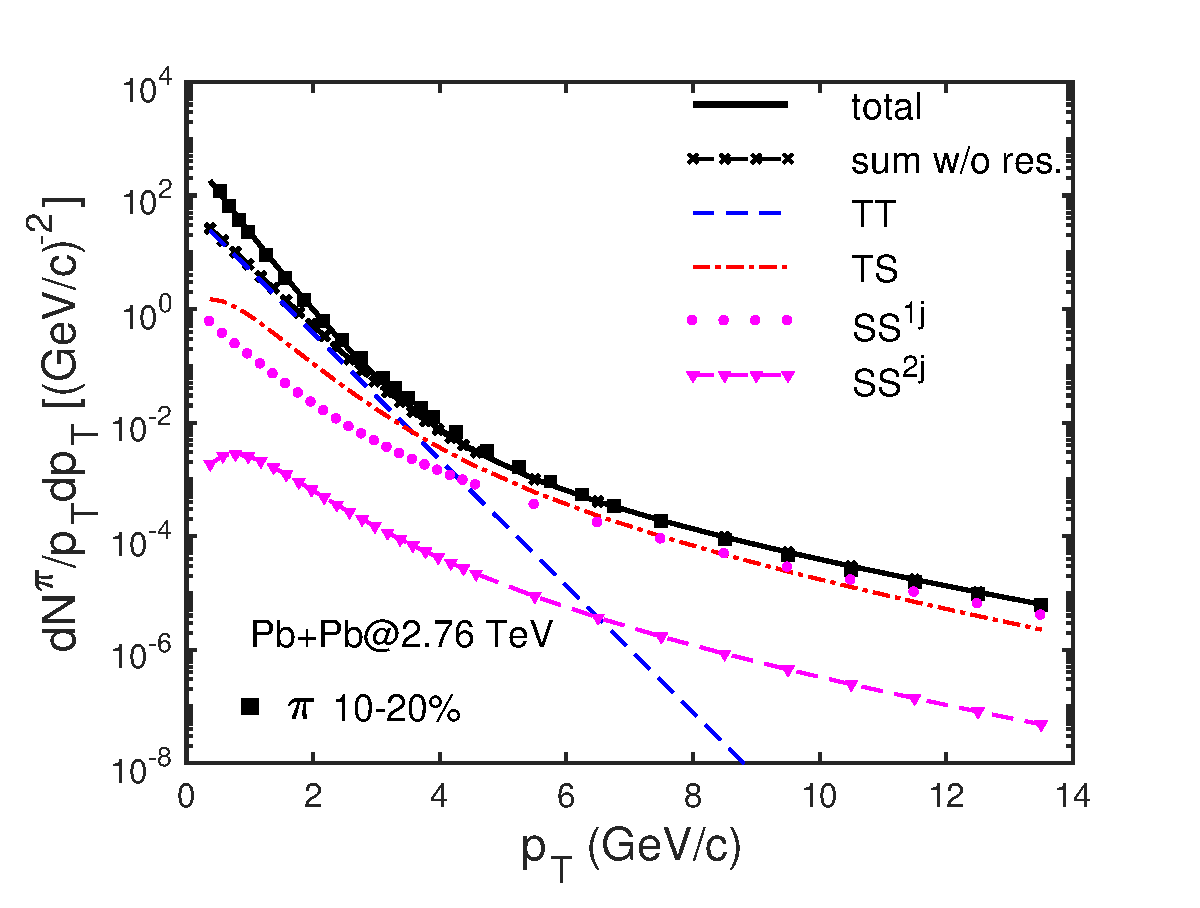
\includegraphics[width=0.45\textwidth]{fig1.eps}
% \caption{(Color online) Transverse momentum spectrum of pion at the centrality of 10-20\% in Pb+Pb collisions at $\sqrt{s_{NN}}=2.76$ TeV. The data are taken from Ref. \cite{Adam:2015kca}.}
% \label{fig3}
%\end{figure}
%
%\begin{figure}[pht]
%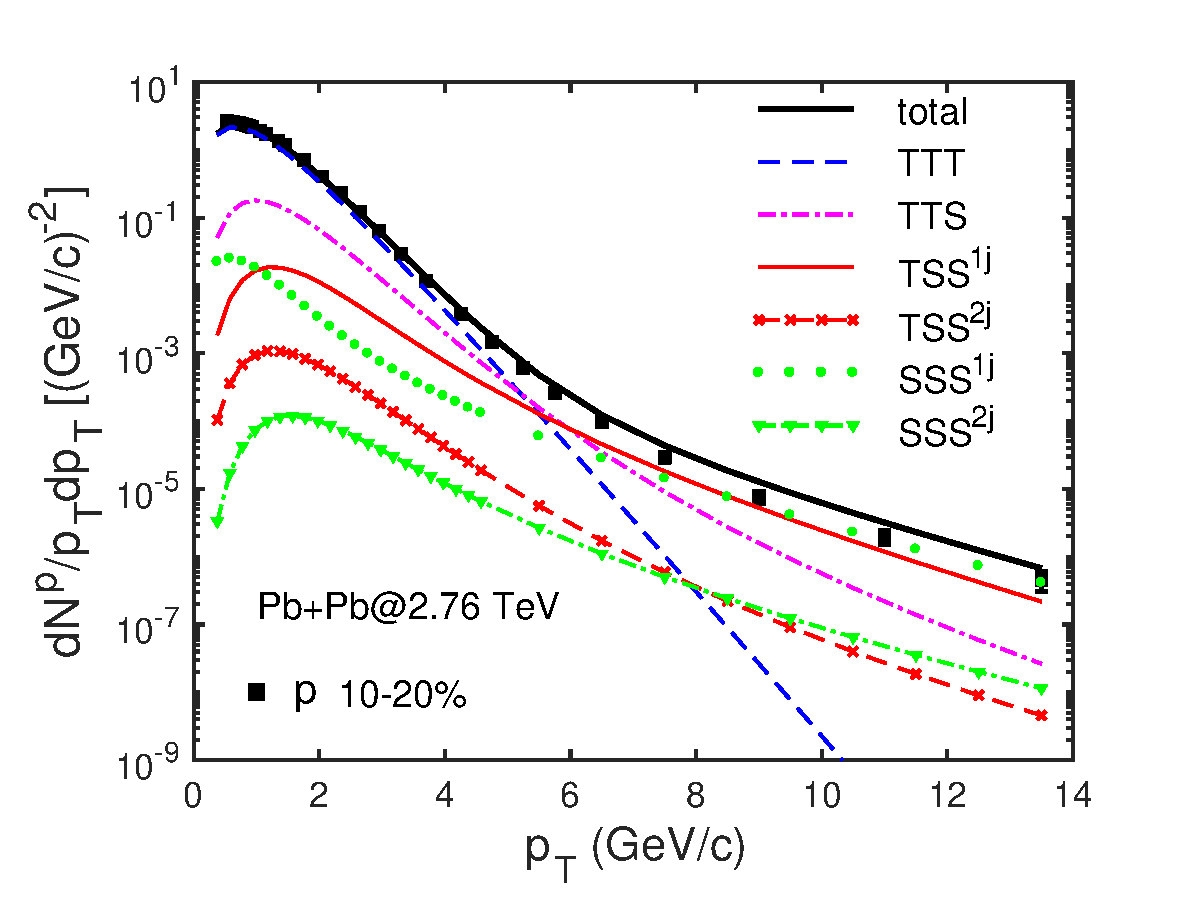
\includegraphics[width=0.45\textwidth]{fig2.eps}
% \caption{(Color online) Transverse momentum spectrum of proton at the centrality of 10-20\% in Pb+Pb collisions at $\sqrt{s_{NN}}=2.76$ TeV. The data are taken from Ref. \cite{Adam:2015kca}.}
% \label{fig4}
%\end{figure}
%
%\subsection{Proton production}
%Proton mass is not negligible, compared to that of pion; thus, $p^0$ in Eq. (\ref{2.2}) should be replaced by the transverse mass $m_T^p=\sqrt{p_T^2+m_p^2}$. The RF for proton is given in Refs. \cite{hy0, hy1, hz1, hz2, Zhu:2014csa}, which includes the momentum conservation $\delta$ function. The thermal-thermal-thermal (TTT) recombination is 
%\begin{eqnarray}
%\frac{dN_p^{TTT}}{p_Tdp_T}=g_{st}^pg_pg_p'\frac{C^3p_T^2}{m_T^p}e^{-p_T/T}, \label{3.7}
%\end{eqnarray}
%where $g_{st}^p=1/6$ and
%\begin{eqnarray}
%g_p=[B(\alpha+1, \alpha+\beta+2)B(\alpha+1, \beta+1)]^{-1}, \label{3.8}
%\end{eqnarray}
%\begin{eqnarray}
%g_p'=B(\alpha+2, \beta+2)B(\alpha+2, \alpha+\beta+4). \label{3.9}
%\end{eqnarray}
%$B(\alpha, \beta)$ is the beta function with $\alpha=1.75$ and $\beta=1.05$.
%
%For thermal-thermal-shower (TTS), thermal-shower-shower (TSS) and shower-shower-shower (SSS) recombination, we have
%\begin{widetext}
%\begin{eqnarray}
%{dN_p^{TTS}\over \pt d\pt}&=&{g_{st}^pg_p C^2\over m_T^p \pt^{2\alpha+\beta+3}} \int_0^{\pt} dp_1 \int_0^{\pt-p_1} dp_2\ e^{-(p_1+p_2)/T}  \left\{ (p_
%_2)^{\alpha+1}(\pt-p_1-p_2)^{\beta} {\cal S}^d(\pt-p_1-p_2, c)\right.\nonumber\\
%&&\left.+p_1^{\alpha+1}p_2^{\beta+1}(\pt-p_1-p_2)^{\alpha} {\cal S}^u(\pt-p_1-p_2, c)\right\}, \label{3.10}
%\end{eqnarray}
%
%\begin{eqnarray}
%{dN_p^{{TSS}^{1j}}\over \pt d\pt}&=&{g_{st}^pg_p C\over m_T^p \pt^{2\alpha+\beta+3}} \int_0^{\pt} dp_1 \int_0^{\pt-p_1} dp_2\ e^{-p_1/T}\left\{ p_1^{\beta+1}p_2^{\alpha}(\pt-p_1-p_2)^{\alpha} {\cal S}^{uu}(p_2,\pt-p_1-p_2, c)\right.\nonumber\\
%&&\left.+p_1(p_1p_2)^{\alpha}(\pt-p_1-p_2)^{\beta} {\cal S}^{ud}(p_2,\pt-p_1-p_2, c)\right\},\label{3.11}
%\end{eqnarray}
%
%\begin{eqnarray}
%{dN_p^{{TSS}^{2j}}\over \pt d\pt}&=&{g_{st}^pg_p  C\Gamma\over m_T^p \pt^{2\alpha+\beta+3}} \int_0^{\pt} dp_1 \int_0^{\pt-p_1} dp_2\ e^{-p_1/T}  \left\{ p_1^{\beta+1}p_2^{\alpha}(\pt-p_1-p_2)^{\alpha} {\cal S}^u(p_2, c) {\cal S}^{u}(\pt-p_1-p_2, c)\right.\nonumber\\
%&&\left.+p_1(p_1p_2)^{\alpha}(\pt-p_1-p_2)^{\beta} {\cal S}^u(p_2, c) {\cal S}^{d}(\pt-p_1-p_2, c)\right\}, \label{3.13}
%\end{eqnarray}
%
%\begin{eqnarray}
%{dN_p^{{SSS}^{1j}}\over \pt d\pt}=\frac{1}{m_T^p}\int\frac{dq}{q^2}\sum\limits_i\hat F_i(q, c)D_i^p(p_T, q),\label{3.12}
%\end{eqnarray}
%
%\begin{eqnarray}
%{dN_p^{{SSS}^{2j}}\over \pt d\pt}&=&{g_{st}^pg_p\Gamma \over m_T^p \pt^{2\alpha+\beta+3}} \int_0^{\pt} dp_1 \int_0^{\pt-p_1} dp_2 \left\{ p_1^{\beta}p_2^{\alpha}(\pt-p_1-p_2)^{\alpha} {\cal S}^d(p_1, c) {\cal S}^{uu}(p_2,\pt-p_1-p_2, c)\right.\nonumber\\
%&&\left.+(p_1p_2)^{\alpha}(\pt-p_1-p_2)^{\beta} {\cal S}^u(p_1, c) {\cal S}^{ud}(p_2,\pt-p_1-p_2, c)\right\}, \label{3.14}
%\end{eqnarray}
%
%where
%\begin{eqnarray}
%\mathcal{S}^{qq}(p_2, p_3, c)=\int\frac{dq}{q}\sum\limits_i\hat F_i(q, c){\rm S}_i^q(p_2, q){\rm S}_i^q(p_3, q-p_2).\label{3.15}
%\end{eqnarray}
%\end{widetext}
%
%\subsection{Kaon production}
%The four components of kaon distribution are very similar to those of pion. The differences are in the constituent quark masses between $m_q$ and $m_s$ resulting in asymmetry of the RF for kaon \cite{hwaprc2007} and the different $T_q$ of light quarks and $T_s$ of $s$ quarks. The kaon production is written as
%%\begin{widetext}
%\begin{eqnarray}
%{dN^{TT}_{K}\over p_Tdp_T} &=&
%{12CC_s\over m_T^Kp_T^5} \int_0^{\pt} dp_1 p_1(\pt-p_1)^2 \nonumber\\
%&&\times p_1e^{-p_1/T}(p_T-p_1)e^{-(p_T-p_1)/T_s} ,     \label{3.16}
%\end{eqnarray}
%
%\begin{eqnarray}
%{dN_{K}^{TS}\over p_Tdp_T} &=& {12\over m_T^Kp_T^5} \int_0^{\pt} dp_1 p_1^2(\pt-p_1)^2\nonumber  \\
%&&\left[Ce^{-p_1/T}{\cal S}^{\bar s}(p_T-p_1,c)\right. \nonumber  \\
%&&\left. +C_s\left({\pt\over p_1}-1\right)e^{-(\pt-p_1)/T_s}{\cal S}^u(p_1,c)\right] ,    \label{3.17} 
%\end{eqnarray}
%
%\begin{eqnarray}
%{dN^{{SS}^{1j}}_{K}\over p_Tdp_T} &=& {1\over m^K_T} \int {dq\over q^2} \sum_i \hat{F}_i(q ,c)D^{K}_i(p_T,q)
%,  \label{3.18}
%\end{eqnarray}
%
%\begin{eqnarray}
%{dN_{K}^{{SS}^{2j}}\over p_Tdp_T} &=& {12\Gamma\over m_T^Kp_T^5} \int_0^{\pt} dp_1 p_1(\pt-p_1)^2  \nonumber  \\
%&&\times{\cal S}^{u}(p_1,c) {\cal S}^{\bar s}(p_T-p_1,c) .    \label{3.19} 
%\end{eqnarray}
%%\end{widetext}
%
% \begin{figure*}[t]
% \centering
%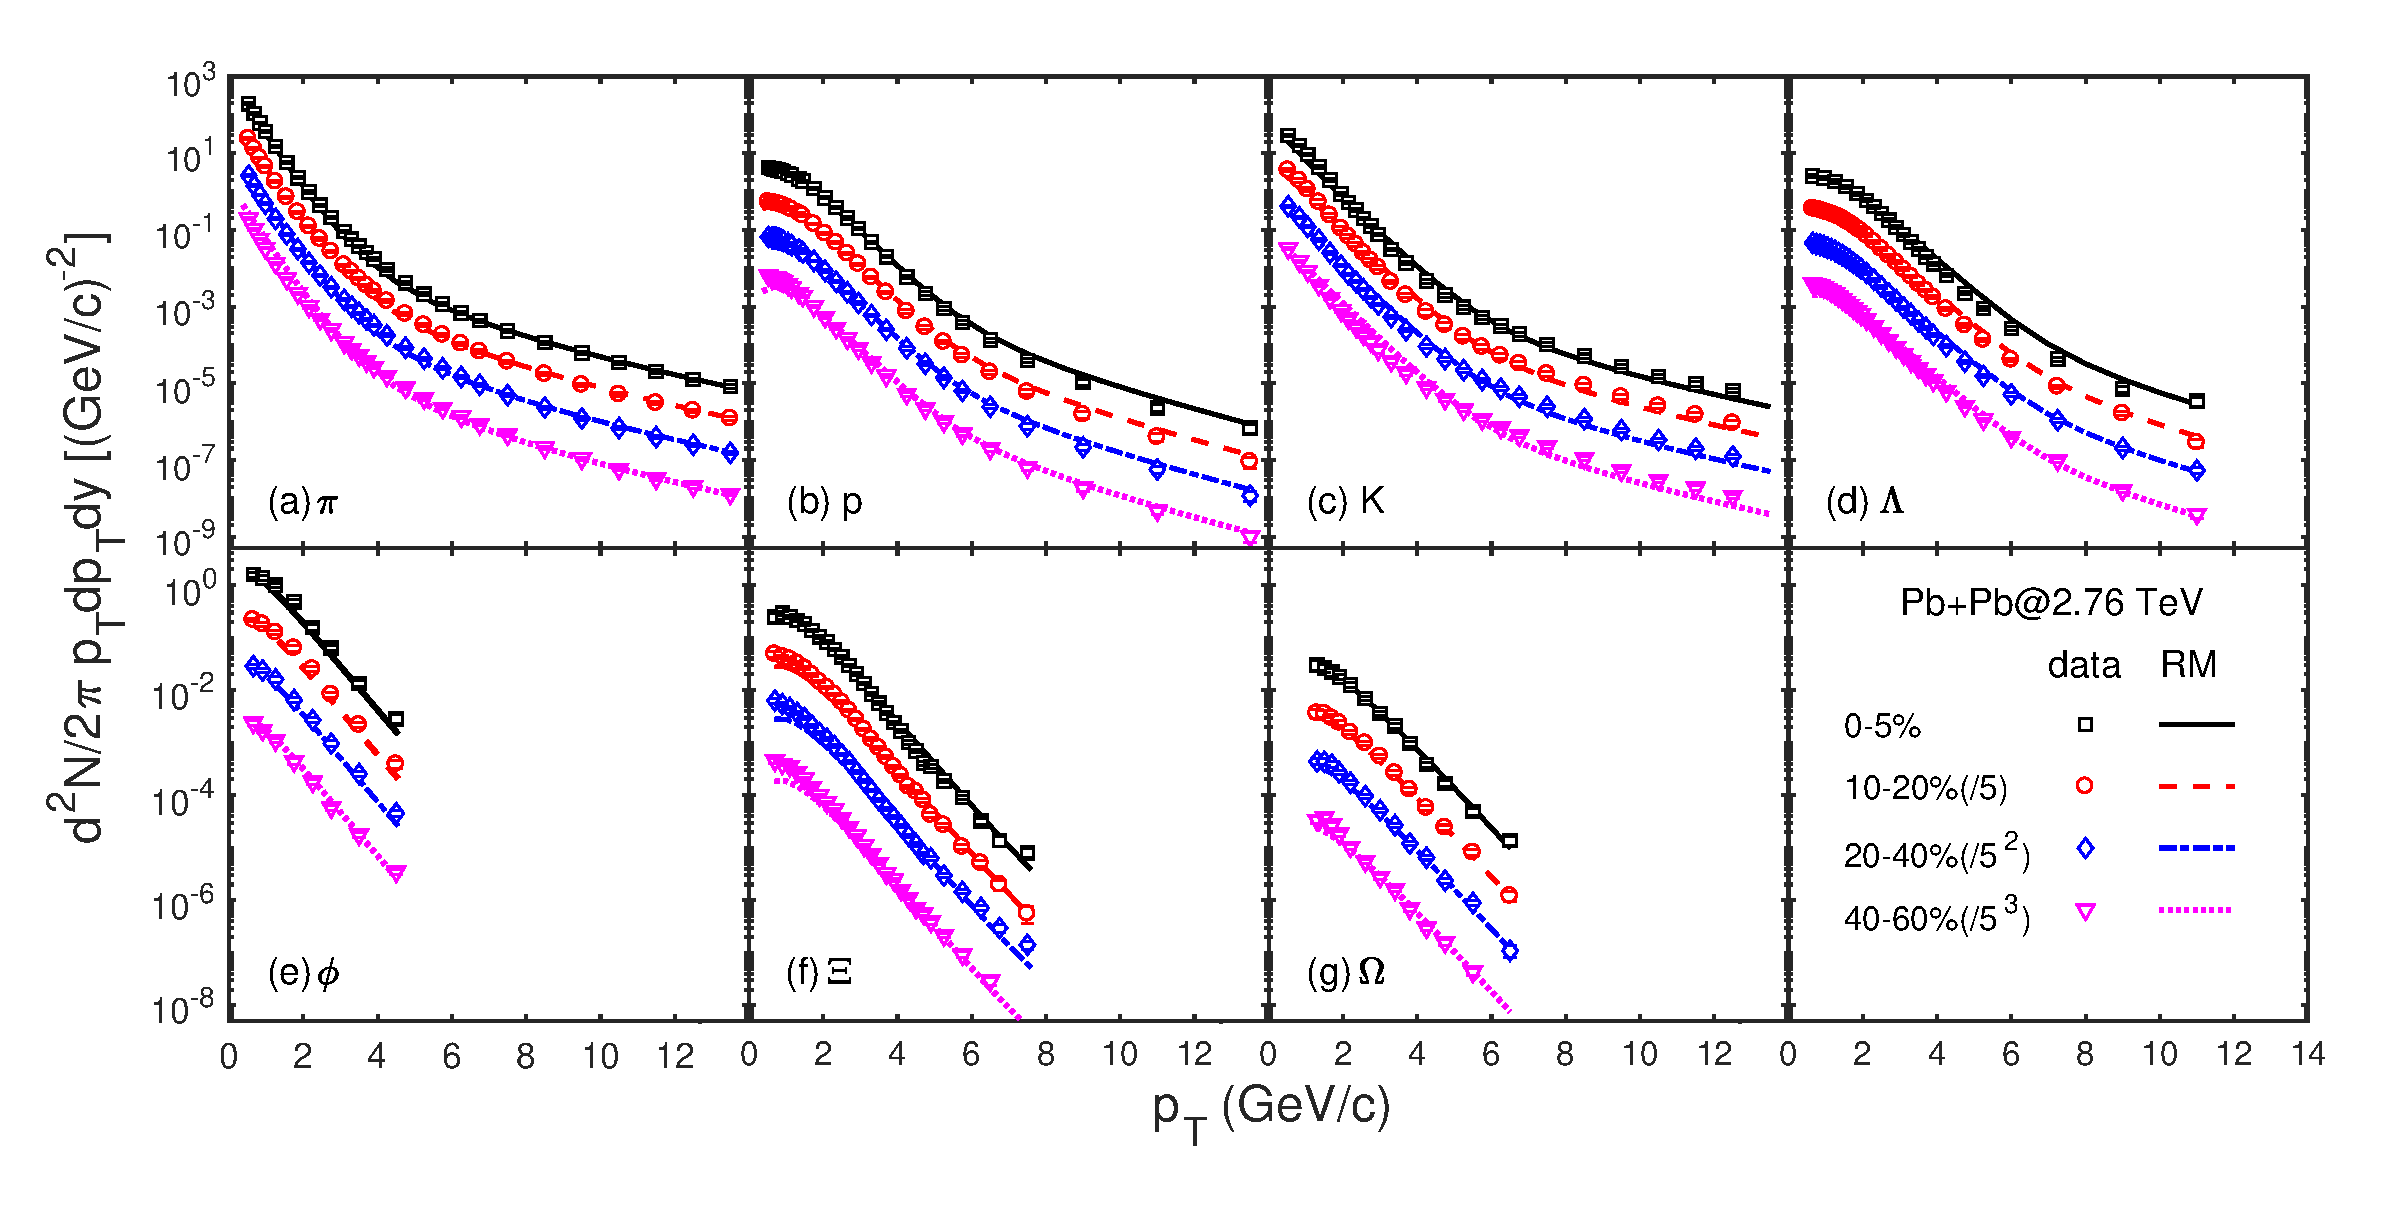
\includegraphics[width=0.9\textwidth]{fig3.eps}
%  \caption{(Color online) Transverse momentum spectra of pion (a), proton (b), kaon (c), $\Lambda$ (d), $\phi$ (e), $\Xi$ (f) and $\Omega$ (g) from the recombination model at midrapidity in Pb+Pb collisions at $\sqrt{s_{NN}}=2.76$ TeV for different centrality classes. Scale factors are applied for better visibility. The data are taken from Ref. \cite{Adam:2015kca} for pion, kaon and proton, Ref. \cite{Abelev:2014uua} for $\phi$,  Ref. \cite{Abelev:2013xaa} for $\Lambda$ and Ref. \cite{ABELEV:2013zaa} for $\Xi$ and $\Omega$.}
%\label{fig5}
%\end{figure*}



\section{transverse momentum distribution of hadrons}\label{DOH4}
As stated above, the two essential coefficient $C_q$ and $C_s$, which corresponds to (u,d) quark and s quark respectively, can be obtained from baryon spectra function of proton ($B_p$) and meson spectra function of $\phi$ ($M_{\phi}$). After the recombination functions(RM) of all the identified hadrons are derived, we summarize the transverse momentum distributions of them explicitly here.
\subsection{Proton production}
The RM for proton is given in Refs.\cite{2u,Zhu:2013cza,Hwa:2002tu,Hwa:2004ng,Hwa:2011bw}, and thus the thermal-thermal-thermal($TTT$) recombination is 
\begin{eqnarray}
\frac{dN_p^{TTT}}{p_Tdp_T}=g_{st}^pg_pg_p'\frac{C_q^3p_T^2}{m_T^p}e^{-p_T/T_q}, \label{4.1}
\end{eqnarray}
where $g_{st}^p=1/6$ and
\begin{eqnarray}
g_p=[B(\alpha+1, \alpha+\beta+2)B(\alpha+1, \beta+1)]^{-1}, \label{4.2}
\end{eqnarray}
\begin{eqnarray}
g_p'=B(\alpha+2, \beta+2)B(\alpha+2, \alpha+\beta+4). \label{4.3}
\end{eqnarray}
$B(\alpha, \beta)$ is the beta function with $\alpha=1.75$ and $\beta=1.05$.
Afterwards, compared with Eq.\ref{3.3}, we multiply Eq.\ref{4.1} by $m_T^p/p_T^2$ to derive $C_q$ shown in Table \ref{tab3} from Eq.\ref{3.6}
\begin{eqnarray}
	C_q(s,N_{part})=[A_{p}(s,N_{part})/g_{st}^p g_p g_p']^{1/3} .\label{4.4}
\end{eqnarray}
The value of $C_q$ is generally consistent with it in Eq.\ref{2.10}. After that, we figure out the transverse momentum distribution of proton by substituting $C_q$ and $T_q$ into Eq.\ref{4.1}.

\subsection{$\phi$ production}
Then, we consider the production of $\phi$. When the RF is taken to be \cite{Hwa:2006vb}
\begin{eqnarray}
R_{s\overline s}(p_1,p_2,p_T)={\text g}_{\phi}p_1p_2 \prod \limits_{i=1}^2\delta(p_i-p_T/2),\label{4.5}
\end{eqnarray}
where $g_{\phi}$=0.432, the distribution for $\phi$ is gained.
\begin{eqnarray}
	\frac{dN_{\phi}^{TT}}{p_Tdp_T}=g_{\phi}\frac{C_s^2p_T}{4m_T^{\phi}}e^{-p_T/T_s}, \label{4.6}
\end{eqnarray}
And similarly we multiply Eq.\ref{4.6} by $m_T^{\phi}/p_T$ to obtain $C_s$ shown in Table \ref{tab4} from Eq.\ref{3.5}
\begin{eqnarray}
C_s(s,N_{part})=[4A_{\phi}(s,N_{part})/g_{\phi}]^{1/2} .\label{4.7}
\end{eqnarray}
Therefore, the distributions for all identified hadrons, including $\phi$, can be calculated since we have the values of $C_q$ and $C_s$ at all centralities and energies.
\begin{table*}[htbp]
		\centering
		\tabcolsep0.25in
		%	\begin{spacing}{1.3}
			\begin{tabular}{cccccc}
				\hline
				\hline
				\diagbox[width=12em]{$\sqrt{s}$(GeV)}{centrality}   &  0-5\%&10-20\%&20-30\%&30-40\%&40-60\%\\
				\hline
				7.7  &  60.7031  & 51.3111 &  44.4750  & 38.4560 &  31.4561\\
				11.5 &  53.3346 &  44.3816  & 38.6098 &  33.1342  & 27.3459\\
				19.6	&  45.5197 &  38.8299  & 33.2419 &  28.0365  & 23.8158\\
				27  &  42.1296 &  35.9997  & 31.3034 &  26.8425  & 22.4945\\
				39   &  38.0702 &  32.7682  & 28.7857 &  24.8077  & 20.8087\\
				\hline
				\hline
			\end{tabular}
		%	\end{spacing}
	\caption{Values of $C_q[(GeV/c)^{-1}]$ at various centralities and energies in Au+Au collision. The values of $N_{part}$ are taken from \cite{STAR:2017sal}.} 
	\label{tab3}
\end{table*}

\begin{table*}[htbp]
	\centering
		\tabcolsep0.25in
		%	\begin{spacing}{1.3}
			\begin{tabular}{cccccc}
				\hline
				\hline
					\diagbox[width=12em]{$\sqrt{s}$(GeV)}{centrality}  &  0-5\%&10-20\%&20-30\%&30-40\%&40-60\%\\
				\hline
				7.7  &  7.6029  &  5.9358  &  4.8195  &  3.7510 &   2.4599\\
				11.5 &  8.6279  &  7.2180  &  5.5505  &  4.1935 &   2.6197\\
				19.6	&  9.4689  &  7.7271  &  6.0909  &  4.9368 &   3.1813\\
				27  &  9.9892  &  8.0698  &  6.5269  &  4.9392 &   3.4590\\
				39   &  9.7526  &  8.1763  &  6.6462  &  5.3283 &   3.4642\\
				\hline
				\hline	
			\end{tabular}
		%	\end{spacing}
	\caption{Values of $C_s[(GeV/c)^{-1}]$  at various centralities and energies in Au+Au collision. The values of $N_{part}$ are taken from \cite{STAR:2017sal}.} 
	\label{tab4}
\end{table*}
\subsection{$\Xi$, $\Lambda$ and $\Omega$ production}
The $p_T$ distributions of $\Xi$, $\Lambda$ and $\Omega$ are quite similar to that of proton. The differences among them are the number of strange quarks in $h$ and the RF for various hadrons. Since the RF for $\Xi$, $\Lambda$ and $\Omega$ have been given in \cite{2u,Hwa:2006vb,Hwa:2011bw}, we have
\begin{eqnarray}
	\frac{dN_{\Xi}^{TTT}}{p_Tdp_T}=\frac{g_{\Xi}C_qC_s^2p_T^2}{27m_T^{\Xi}}e^{-p_T/3T_q}e^{-2p_T/3T_s}, \label{4.8}
\end{eqnarray}
where $g_{\Xi}$=0.03,
\begin{eqnarray}
\frac{dN_{\Lambda}^{TTT}}{p_Tdp_T}&=&g_{st}^{\Lambda}N_{\Lambda}[B(\alpha+2,\beta+2)B(\alpha+2,\alpha+\beta+4)]\nonumber\\
&&\frac{C_q^2C_sp_T^2}{m_T^{\Lambda}}e^{-2p_T/3T_q}e^{-p_T/3T_s}, 
\label{4.9}
\end{eqnarray}
where $g_{st}^{\Lambda}$=1/8(1/2 for $\Lambda^0$ or $\Sigma^0$, and 2/8 from spin consideration) and the RF parameters for $\Lambda$ are $\alpha$=1, $\beta$=2, and
\begin{eqnarray}
		\frac{dN_{\Omega}^{TTT}}{p_Tdp_T}=\frac{g_{\Omega}C_s^3p_T^2}{27m_T^{\Omega}}e^{-p_T/T_s}, \label{4.10}
\end{eqnarray}
where $g_{\Omega}$=0.01. 

\section{results}\label{results5}
So far, we have presented the equations of the five hadronic spectra. As for $\pi$ and K, the contribution from the resonance decays must be considered, which is taken into account in Fig.\ref{fig1} and not interested here. For thermal partons, the inverse slopes $T$ and $T_s$ are independent of centrality, so the free parameters are just the centrality dependence of normalization factors, $C_q$ and $C_s$\cite{3c}.

The results from RM in Au+Au collisions for five identified hadrons, i.e.,p, $\Lambda$, $\phi$, $\Xi$ and $\Omega$, are shown in Figs.\ref{fig9}$\sim$\ref{fig13}. All centralities and five energies at BES region are taken into account. Data are from Refs.\cite{STAR:2019bjj,STAR:2017sal,STAR:2015vvs}. The dashed lines from calculations reproduce the $p_T$ distributions well in general throughout the whole region where data exist. In addition, we predict the spectra of $\Omega$ in central and non-central Au+Au collisions at $\sqrt{s}$=7.7, 11.5 GeV with recombination model, which can be testified in the future.

 All the experimental value/theoretical value ratios are limited within 1.5. Although the ratios do not show the perfect agreement, it is a significant achievement to get a good fit over wide ranges of $p_T$ for all the identified hadrons at various centralities in quite a wide collision energy. Accordingly, it is deduced that recombination model is a excellent approach to describe the transverse momentum and centrality dependence of hadron production in the nuclear collisions. 
\begin{figure*}[pht]
	\includegraphics[width=0.9\textwidth]{pic9.png}
	\caption{(colored online)Transverse momentum spectra of proton (a), $\Lambda$ (b), $\Xi$ (c), $\Omega$ (d) and $\phi$ (e) for Au+Au collisions at $\sqrt{s_{NN}}=7.7$ GeV and various centralities. The experimental value/theoretical value ratios lie in the bottom of each subfigure. The experimental data are taken from Refs. \cite{STAR:2019bjj,STAR:2017sal,STAR:2015vvs}.}
	\label{fig9}
\end{figure*}
\begin{figure*}[pht]
	\includegraphics[width=0.9\textwidth]{pic10.png}
	\caption{(colored online)Transverse momentum spectra of proton (a), $\Lambda$ (b), $\Xi$ (c), $\Omega$ (d) and $\phi$ (e) for Au+Au collisions at $\sqrt{s_{NN}}=11.5$ GeV and various centralities. The experimental value/theoretical value ratios lie in the bottom of each subfigure. The experimental data are taken from Refs. \cite{STAR:2019bjj,STAR:2017sal,STAR:2015vvs}.}
	\label{fig10}
\end{figure*}
\begin{figure*}[pht]
	\includegraphics[width=0.9\textwidth]{pic11.png}
	\caption{(colored online)Transverse momentum spectra of proton (a), $\Lambda$ (b), $\Xi$ (c), $\Omega$ (d) and $\phi$ (e) for Au+Au collisions at $\sqrt{s_{NN}}=19.6$ GeV and various centralities. The experimental value/theoretical value ratios lie in the bottom of each subfigure. The experimental data are taken from Refs. \cite{STAR:2019bjj,STAR:2017sal,STAR:2015vvs}.}
	\label{fig11}
\end{figure*}
\begin{figure*}[pht]
	\includegraphics[width=0.9\textwidth]{pic12.png}
	\caption{(colored online)Transverse momentum spectra of proton (a), $\Lambda$ (b), $\Xi$ (c), $\Omega$ (d) and $\phi$ (e) for Au+Au collisions at $\sqrt{s_{NN}}=27$ GeV and various centralities. The experimental value/theoretical value ratios lie in the bottom of each subfigure. The experimental data are taken from Refs. \cite{STAR:2019bjj,STAR:2017sal,STAR:2015vvs}.}
	\label{fig12}
\end{figure*}
\begin{figure*}[pht]
	\includegraphics[width=0.9\textwidth]{pic13.png}
	\caption{(colored online)Transverse momentum spectra of proton (a), $\Lambda$ (b), $\Xi$ (c), $\Omega$ (d) and $\phi$ (e) for Au+Au collisions at $\sqrt{s_{NN}}=39$ GeV and various centralities. The experimental value/theoretical value ratios lie in the bottom of each subfigure. The experimental data are taken from Refs. \cite{STAR:2019bjj,STAR:2017sal,STAR:2015vvs}.}
	\label{fig13}
\end{figure*}
\section{valon-recombination model}\label{VM6}
Aiming at the slight deviation for $p_T$ distribution of kaon in Fig.\ref{fig1}(g), we pay attention to the valon-recombination model(VRM)\cite{5i,Hwa:2002mv,Hwa:2001ih,Hwa:1980mv,Hwa:1980xv}. In the quark model suitable for describing deep-inelastic scattering process by CTEQ\cite{Hwa:2002mv}, there are three valence quarks plus an infinity of sea quarks and gluons\cite{Hwa:1980xv}, and we shall regarded these clusters as valons. Each valon has a valence quark, as well as its own sea quarks and gluons, playing a role in the collision problem as the constituent quarks do in the bound-state problem\cite{Hwa:2001ih}. The valon model has been studied in p-p and p-A collisions when the CTEQ data and p-Pb data in the NA49 experiment are published previously. Now we attempt to generalize VRM to A-A collisions. Firstly we need a rough assumption, in which one of the two targets is decomposed into the single valons so that we can calculate momentum distribution for proton from the available results\cite{Hwa:2001ih} in p-A collisions.

Let us begin with the invariant distribution function for the detection of a proton at momenta fraction x is 
\begin{eqnarray}
	H_p(x)&=&\frac{1}{N}\int \frac{dx_1}{x_1}\frac{dx_2}{x_2}\frac{dx_3}{x_3}F(x_1,x_2,x_3)\nonumber\\
	&&\times R_p(x_1,x_2,x_3,x),
	\label{6.1}
\end{eqnarray}
where $N$ is the normalization factor. Note the two invariant distributions: $F(x_1,x_2,x_3)$ denotes the probability of finding a u quark at $x_1$, another u quark at $x_2$, and a d quark at $x_3$, and $R_p(x_1,x_2,x_3,x)$ denotes the recombination function, which specifies the probability that those three quarks coalesce to form a proton at $x$.

The quark distribution from the proton is 
\begin{eqnarray}
	F_p(x_1,x_2,x_3)&=&\int dy'_1dy'_2dy'_3G'_{\overline v}(y'_1,y'_2,y'_3)\nonumber\\
	&&\times M_p(y'_1,y'_2,y'_3;x_1,x_2,x_3),
	\label{6.2}
\end{eqnarray}
where $G'_{\overline v}$ is associated with the valon distribution after momentum degradation and $M_p$ denotes various types of recombination from quarks in valons to identified hadrons, which are all given in \cite{Hwa:2001ih}. Similarly, we can get anti-proton distribution function $H_{\overline p}(x)$, after which we obtain the final formula for net proton production
\begin{eqnarray}
	H_{p-\overline p}(x)=H_p(x)-H_{\overline p}(x).\label{6.3}
\end{eqnarray}
Following by the notion above, the momentum distribution for kaon is available.

\section{conclusion}\label{summary7}
In this paper, we have studied seven identified hadron spectra in the recombination model in Au+Au collisions at beam energy region at RHIC. The theoretical results reproduce the experimental data very well at $\sqrt{s}$=7.7, 11.5, 19.6, 27, 39 GeV and all centralities. Moreover, we figure out the universal exponential features without model input by defining the baryon and meson spectra functions, and then we derive the parameters $C_j(s,N_{part})$ at BES region.

Finally, Considering the slight deviation of spectra for K, we come up with the valon-recombination model that had been studied previously. Although the VRM in A-A collisions is under intensive exploration, it can be expected to improve the theoretical curve to fit data in the future.

With the previous work\cite{3c,4u}, the successful agreement with available data in the framework of the recombination model indicates that the recombination model work well at such a wide range of $\sqrt{s}$=7.7 GeV$\sim$5.02 TeV. Therefore, we can conclude that the recombination model is one of the optimal approaches to describe the hadronic production in high energy collisions.


\section*{Acknowledgements}




\begin{thebibliography}{99}

%\cite{STAR:2015vvs}
\bibitem{STAR:2015vvs}
L.~Adamczyk \textit{et al.} [STAR],
%``Probing parton dynamics of QCD matter with $\Omega$ and $\phi$ production,''
Phys. Rev. C \textbf{93}, no.2, 021903 (2016)
doi:10.1103/PhysRevC.93.021903
[arXiv:1506.07605 [nucl-ex]].
%43 citations counted in INSPIRE as of 07 Dec 2021

\bibitem{2u}
%A unified study of the production of all identified hadrons over wide ranges of transverse momenta at LHC
Lilin Zhu and Rudolph C Hwa 2020 {\it J. Phys. G: Nucl. Part. Phys.} {\bf 47} 055102

\bibitem{3c}
%828-v3 Centrality and transverse momentum dependence of hadrons in Pb+Pb collisions at LHC
Lilin Zhu, Hua Zheng and Rudolph C Hwa 2020, Phys.\ Rev.\ C {\bf 104}, 014902 

\bibitem{4u}
%Universal formula for baryon spectra in heavy-ion collisions and its implications
Rudolph C Hwa and Lilin Zhu, Phys.\ Rev.\ C {\bf 97}, 054908 (2018)

\bibitem{5i}
%Inclusive distributions for hadronic collisions in the valon-recombination model
R.~C.~Hwa and C.~B.~Yang, Phys.\ Rev.\ C {\bf 66}, 025205(2002)

\bibitem{6c}
R.~C.~Hwa and C.~B.~Yang,
%``Centrality dependence of baryon and meson momentum distributions in proton nucleus collisions,''
Phys. Rev. C \textbf{65}, 034905 (2002)
[erratum: Phys. Rev. C \textbf{67}, 059902 (2003)]
doi:10.1103/PhysRevC.67.059902
[arXiv:nucl-th/0108043 [nucl-th]].
%22 citations counted in INSPIRE as of 05 Dec 2021

%\cite{STAR:2019bjj}
\bibitem{STAR:2019bjj}
J.~Adam \textit{et al.} [STAR],
%``Strange hadron production in Au+Au collisions at $\sqrt{s_{NN}}=$7.7 , 11.5, 19.6, 27, and 39 GeV,''
Phys. Rev. C \textbf{102}, no.3, 034909 (2020)
doi:10.1103/PhysRevC.102.034909
[arXiv:1906.03732 [nucl-ex]].
%37 citations counted in INSPIRE as of 07 Dec 2021

%\cite{STAR:2017sal}
\bibitem{STAR:2017sal}
L.~Adamczyk \textit{et al.} [STAR],
%``Bulk Properties of the Medium Produced in Relativistic Heavy-Ion Collisions from the Beam Energy Scan Program,''
Phys. Rev. C \textbf{96}, no.4, 044904 (2017)
doi:10.1103/PhysRevC.96.044904
[arXiv:1701.07065 [nucl-ex]].
%353 citations counted in INSPIRE as of 07 Dec 2021

%\cite{Hwa:2002mv}
\bibitem{Hwa:2002mv}
R.~C.~Hwa and C.~B.~Yang,
%``Parton distributions in the valon model,''
Phys. Rev. C \textbf{66}, 025204 (2002)
doi:10.1103/PhysRevC.66.025204
[arXiv:hep-ph/0202140 [hep-ph]].
%58 citations counted in INSPIRE as of 08 Dec 2021

%\cite{Zhu:2013cza}
\bibitem{Zhu:2013cza}
L.~Zhu and R.~C.~Hwa,
%``Centrality and Transverse Momentum Dependencies of Minijets and Hadrons in Au-Au Collisions,''
Phys. Rev. C \textbf{88}, no.4, 044919 (2013)
doi:10.1103/PhysRevC.88.044919
[arXiv:1307.3328 [nucl-th]].
%7 citations counted in INSPIRE as of 02 Jan 2022

%\cite{Hwa:2002tu}
\bibitem{Hwa:2002tu}
R.~C.~Hwa and C.~B.~Yang,
%``Scaling behavior at high p(T) and the p / pi ratio,''
Phys. Rev. C \textbf{67}, 034902 (2003)
doi:10.1103/PhysRevC.67.034902
[arXiv:nucl-th/0211010 [nucl-th]].
%349 citations counted in INSPIRE as of 02 Jan 2022

%\cite{Hwa:2004ng}
\bibitem{Hwa:2004ng}
R.~C.~Hwa and C.~B.~Yang,
%``Recombination of shower partons at high p(T) in heavy ion collisions,''
Phys. Rev. C \textbf{70}, 024905 (2004)
doi:10.1103/PhysRevC.70.024905
[arXiv:nucl-th/0401001 [nucl-th]].
%247 citations counted in INSPIRE as of 02 Jan 2022

%\cite{Hwa:2011bw}
\bibitem{Hwa:2011bw}
R.~C.~Hwa and L.~Zhu,
%``Spectra of Identified Hadrons in Pb-Pb Collisions at LHC,''
Phys. Rev. C \textbf{84}, 064914 (2011)
doi:10.1103/PhysRevC.84.064914
[arXiv:1109.6300 [nucl-th]].
%15 citations counted in INSPIRE as of 02 Jan 2022

%\cite{Hwa:2006vb}
\bibitem{Hwa:2006vb}
R.~C.~Hwa and C.~B.~Yang,
%``Production of strange particles at intermediate pT in central Au+Au collisions at high energies,''
Phys. Rev. C \textbf{75}, 054904 (2007)
doi:10.1103/PhysRevC.75.054904
[arXiv:nucl-th/0602024 [nucl-th]].
%87 citations counted in INSPIRE as of 03 Jan 2022

%\cite{Hwa:2001ih}
\bibitem{Hwa:2001ih}
R.~C.~Hwa and C.~B.~Yang,
%``Centrality dependence of baryon and meson momentum distributions in proton nucleus collisions,''
Phys. Rev. C \textbf{65}, 034905 (2002)
[erratum: Phys. Rev. C \textbf{67}, 059902 (2003)]
doi:10.1103/PhysRevC.67.059902
[arXiv:nucl-th/0108043 [nucl-th]].
%22 citations counted in INSPIRE as of 04 Jan 2022

%\cite{Hwa:1980mv}
\bibitem{Hwa:1980mv}
R.~C.~Hwa and M.~S.~Zahir,
%``Parton and Valon Distributions in the Nucleon,''
Phys. Rev. D \textbf{23}, 2539 (1981)
doi:10.1103/PhysRevD.23.2539
%99 citations counted in INSPIRE as of 04 Jan 2022

%\cite{Hwa:1980xv}
\bibitem{Hwa:1980xv}
R.~C.~Hwa,
%``The Role of Valons in Low $p_T$ Physics,''
LA-UR-80-2235.
%0 citations counted in INSPIRE as of 04 Jan 2022
\end{thebibliography}

\end{document}




